\documentclass[a4paper,12pt]{book}

\usepackage{url}
\usepackage[brazil]{babel}
\usepackage[pdftex]{graphicx}
\usepackage[pdftex]{hyperref}
\usepackage{float}

\title{Xadrez em Realidade Aumentada \thanks{Obrigado a Daniel Vargas da FATEC - S\~ao Caetano pelos modelos 3D de pe\c cas.}}
\author{
		Douglas Bettioli Barreto (NUSP 6920223)
		\and Giancarlo Rigo (NUSP 6910034)
		\and Rafael Reggiani Manzo (NUSP 6797150)
	   }

\begin{document}

\maketitle

\part{Considera\c c\~oes gerais}
\label{part:consideracoesgerais}
  \chapter{B\'asico}
  \label{chbasico}
  \section{Compila\c c\~ao}
	\label{sec:cgcompilacao}
	Este software foi desenvolvido e testado em Linux Ubuntu 10.04 (32 bits). Mas,
	teoricamente, deve funcionar em qualquer m\'aquina que atenda aos requisitos
	(\ref{subsec:cgrequisitos})
	
	\subsection{Requisitos}
	\label{subsec:cgrequisitos}
    \subsubsection{Usu\'ario}
    \label{subsubsec:requsuario}
    \begin{itemize}
      \item{Shockwave Flash 10.0 r45}
      \item{Webcam}
      \item{Marcadores impressos}
      \item{Tabuleiro de xadrez compat\'ivel com os marcadores}
    \end{itemize}
  
    \subsubsection{Desenvolvedor}
    \label{subsubsec:reqdesenvolvedor}
	  \begin{itemize}
      \item{Shockwave Flash 10.0 r45 (Debug)}
		  \item{Adobe Flex Compiler (mxmlc) Version 4.1.0 build 16076}
	  \end{itemize}
	
	\subsection{Makefile}
	Encontrado dentro da pasta src. Dentro dele substitua o caminho para o mxmlc do
	seu Flex SDK.
	Existem duas op\c c\~oes de debug:
	\begin{itemize}
	  \item{Compilar a vers\~ao de produ\c c\~ao: ``make''}
	  \item{Compilar a vers\~ao de debug: ``make debug''}
	\end{itemize}

\part{Manual do usu\'ario}
\label{part:manualdousuario}
	\chapter{Introdu\c c\~ao}
	Neste manual voc\^e encontrar\'a todas as informa\c c\~oes necess\'arias desde preparar o ambiente (\ref{ch:ambiente}) para o jogo at\'e quais s\~ao os comandos dispon\'iveis durante o jogo. Mas n\~ao tem o objetivo de ensinar xadrez.

  \chapter{Ambiente}
  \label{ch:ambiente}
  A configura\c c\~ao do ambiente para o jogo envolve v\'arios fatores como ilumina\c c\~ao (\ref{sec:iluminacao}), posicionamento dos marcadores (\ref{sec:marcadores}) corretamente e da c\^amera (\ref{sec:posicionamentodacamera}).
    \section{Ilumina\c c\~ao}
    \label{sec:iluminacao}
    Para uma boa identifica\c c\~ao de marcadores, prefira ambientes com luz natural e nunca posicione a c\^amera de frente ao ponto de luz.

    \section{Marcadores}
    \label{sec:marcadores}
      \subsection{O que cada marcador representa}
      \label{subsec:marcadorreprsenta}
        \subsubsection{Marcadores de 0 a 2}
        \label{subsubsec:marcadores0a2}
        Estes marcadores servem para que o software seja capaz de delimitar seu tabuleiro de xadrez.

        Imaginando que sua c\^amera esteja exatamente de frente para o tabuleiro (o que n\~ao \'e o correto para uma boa jogabilidade). O marcador 0 deve estar no canto esquerdo inferior do tabuleiro, 1 deve esta no canto direito inferior e o 2 no canto esquerdo superior.

        Voc\^e vai saber que estes marcadores est\~ao sendo identificados quando aparecerem cubos de m\'armore sobre estes marcadores. Estes s\~ao os marcadores mais importantes e sem eles voc\^e n\~ao poder\'a jogar.

        \subsection{Marcadores de 4 a 11}
        \label{subsubsec:marcadores4a11}
        Representam os peo\~oes brancos, com os quais voc\^e vai jogar.

        \subsection{Marcadores de 12 a 13}
        \label{subsubsec:marcadores12a13}
        Representam as torres brancas, com as quais voc\^e vai jogar.

        \subsection{Marcadores de 14 a 15}
        \label{subsubsec:marcadores14a15}
        Representam os cavalos brancos, com os quais voc\^e vai jogar.
 
        \subsection{Marcadores de 16 a 17}
        \label{subsubsec:marcadores16a17}
        Representam os bispos brancos, com os quais voc\^e vai jogar.

        \subsection{Marcador 18}
        \label{subsubsec:marcador18}
        Representa a rainha branca, com a qual voc\^e vai jogar.

        \subsection{Marcador 19}
        \label{subsubsec:marcador19}
        Representam o rei branco, com o qual voc\^e vai jogar.

    \section{Posicionamento da c\^amera}
    \label{sec:posicionamentodacamera}
    O mais importante sobre a c\^amera \'e que ela sempre deve estar capturando e identificando os tr\^es marcadores delimitadores do tabuleiro (ver \ref{subsubsec:marcadores0a2}).

    Para uma boa experi\^encia de jogo com rela\c c\~ao \`a estabilidade dos marcadores e visualiza\c c\~ao dos modelos 3D, recomendamos que a c\^amera seja posicionada na diagonal do tabuleiro onde fica o marcador 1.

  \chapter{Comandos dispon\'ives no jogo}
  \label{ch:comandosdisponiveisnojogo}
    \section{Confirmar jogada}
    \label{sec:confirmarjogada}
    Toda vez que mover um marcador, para confirmar sua jogada, pressione espa\c co.

    \section{Desfazer a \'ultima jogada}
    \label{sec:desfazeraultimajogada}
    Se, por acaso, o software equivocou-se ao reconhecer sua \'ultima jogada ou voc\^e apenas mudou de id\'eia, pressione Ctrl+Z e sua o tabuleiro voltar\'a para seu estado anterior (aten\c c\~ao, este recurso s'o permite volta para o estado imediatamente anterior).

    \section{Ajuda}
    \label{sec:ajuda}
      Em qualquer momento dentro do jogo, voc\^e pode pressionar H e visualizar uma tela de ajuda, com estas informa\c c\~oes resumidas.
     
\part{Manual do Desenvolvedor}
\label{part:manualdodesenvolvedor}
	\chapter{Diagrama de classes}
	\label{ch:diagramadeclasses}
	\begin{figure}[H]
	\centering
	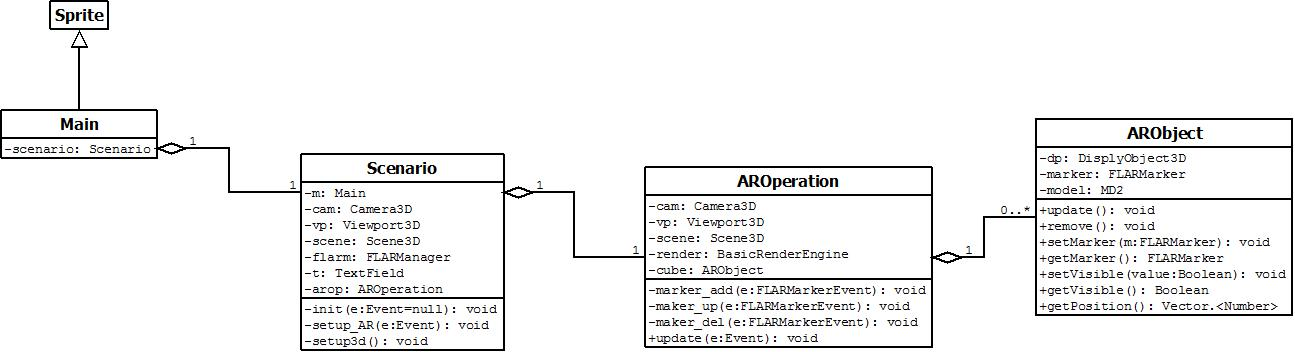
\includegraphics[width=0.7\textwidth, height=0.7\textheight]{diagramadeclasses}
	\end{figure}
	\footnote{Ver observacoes sobre a clase AROperation em
			  \ref{subsec:ecclassearoperation}
			 }

  \chapter{CRC cards}
  \label{ch:crccards}
  \section{Pacote Principal}
	\label{sec:crcpacoteprincipal}
    \subsection{Main}
    \label{subsec:crcmain}
    \begin{figure}[H]
	  \centering
	  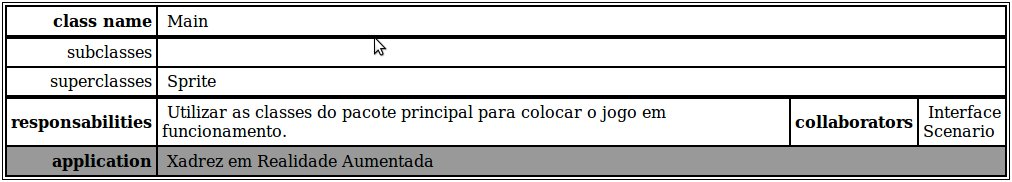
\includegraphics[width=1.0\textwidth]{crc/Main}
	  \end{figure}
  	\subsection{Scenario}
    \label{subsec:crcscenario}
    \begin{figure}[H]
	  \centering
	  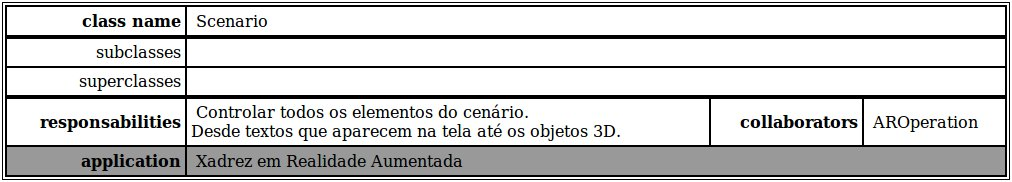
\includegraphics[width=1.0\textwidth]{crc/Scenario}
	  \end{figure}
  	\subsection{Player}
    \label{subsec:crcplayer}
    \begin{figure}[H]
	  \centering
	  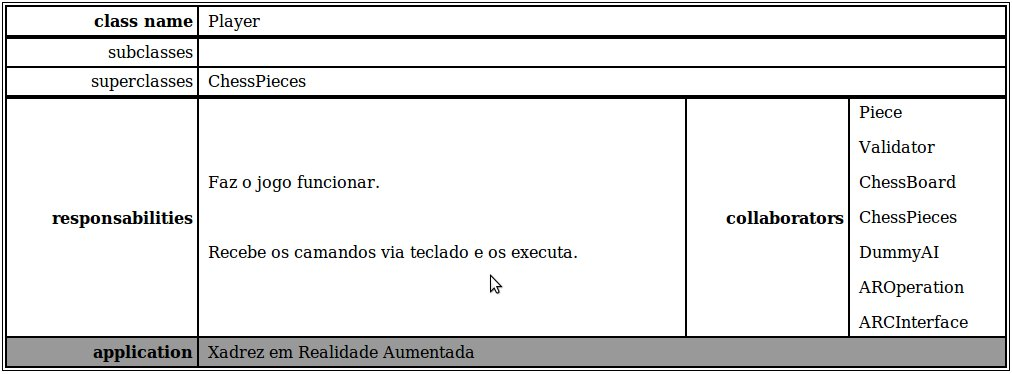
\includegraphics[width=1.0\textwidth]{crc/Player}
	  \end{figure}
  	\subsection{HelpScreen}
    \label{subsec:crchelpscreen}
    \begin{figure}[H]
	  \centering
	  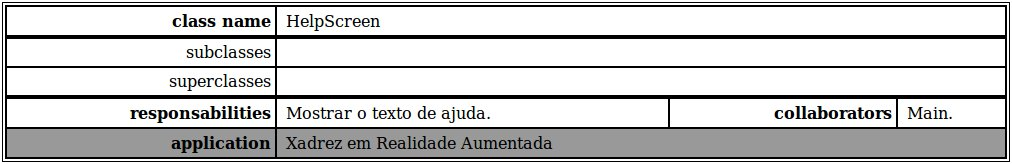
\includegraphics[width=1.0\textwidth]{crc/HelpScreen}
	  \end{figure}
  \section{Pacote AugmentedReality}
  \label{sec:crcpacoteaugmentedreality}
    \subsection{ARCronometer}
    \label{subsec:crcarcronometer}
    \begin{figure}[H]
	  \centering
	  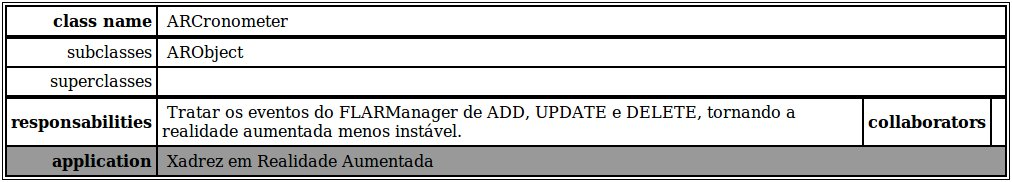
\includegraphics[width=1.0\textwidth]{crc/ARCronometer}
	  \end{figure}
    \subsection{ARObject}
    \label{subsec:crcarobject}
    \begin{figure}[H]
	  \centering
	  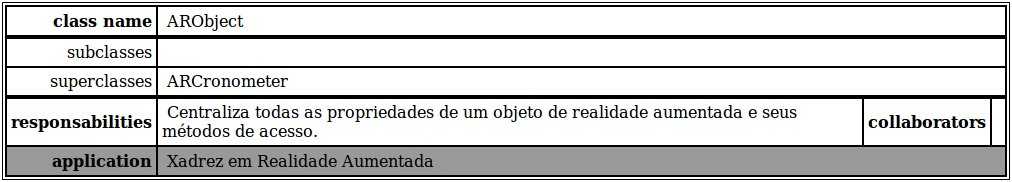
\includegraphics[width=1.0\textwidth]{crc/ARObject}
	  \end{figure}
    \subsection{ARIndependentObject}
    \label{subsec:crcarindependentobject}
    \begin{figure}[H]
	  \centering
	  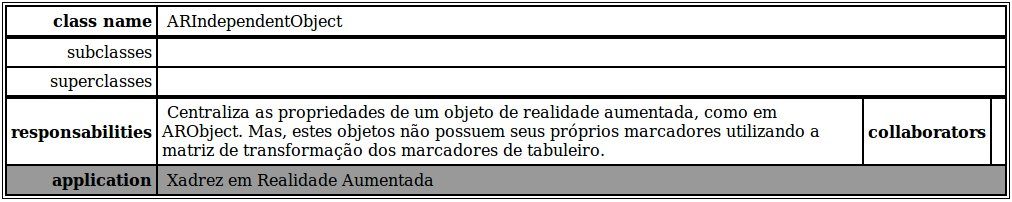
\includegraphics[width=1.0\textwidth]{crc/ARIndependentObject}
	  \end{figure}
    \subsection{AROperation}
    \label{subsec:crcaroperation}
    \begin{figure}[H]
	  \centering
	  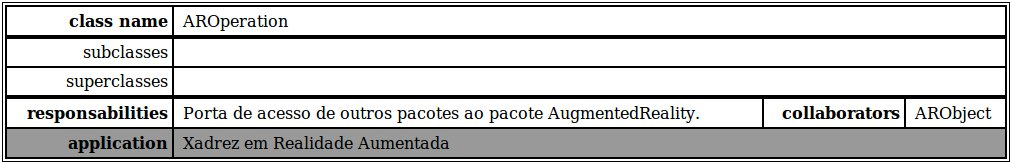
\includegraphics[width=1.0\textwidth]{crc/AROperation}
	  \end{figure}
    \subsection{ARIndependentObject}
    \label{subsec:crcarindependentobject}
    \begin{figure}[H]
	  \centering
	  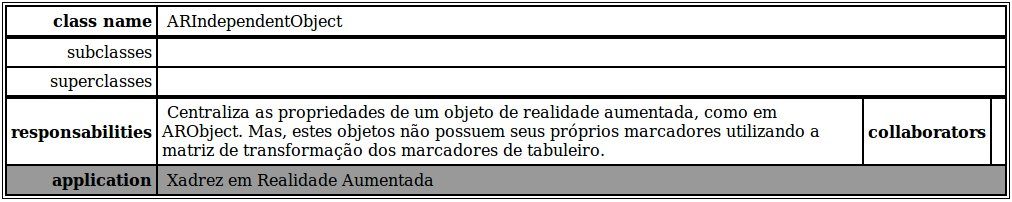
\includegraphics[width=1.0\textwidth]{crc/ARIndependentObject}
	  \end{figure}
  \section{Pacote Game}
  \label{sec:crcpacotegame}
    \subsection{PieceType}
    \label{subsec:crcpiecetype}
    \begin{figure}[H]
	  \centering
	  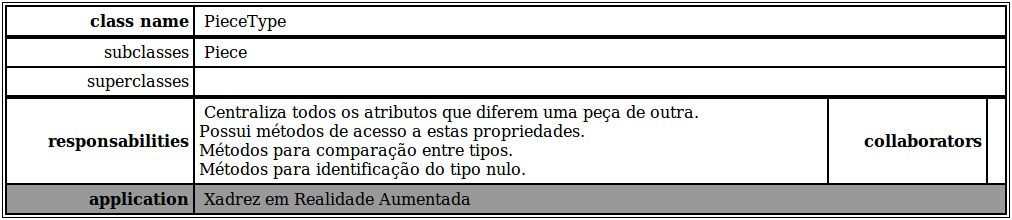
\includegraphics[width=1.0\textwidth]{crc/PieceType}
	  \end{figure}
    \subsection{Piece}
    \label{subsec:crcpiece}
    \begin{figure}[H]
	  \centering
	  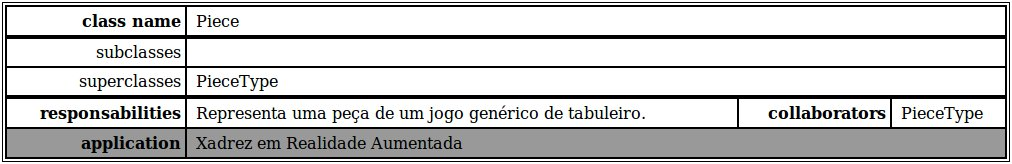
\includegraphics[width=1.0\textwidth]{crc/Piece}
	  \end{figure}
    \subsection{Board}
    \label{subsec:crcboard}
    \begin{figure}[H]
	  \centering
	  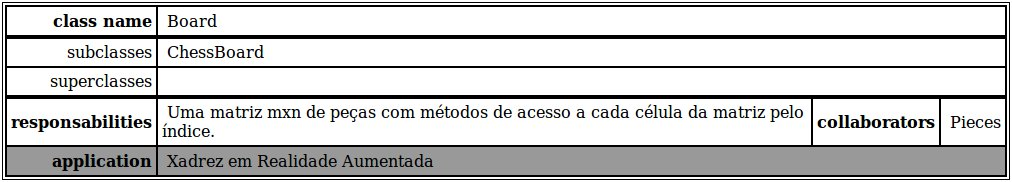
\includegraphics[width=1.0\textwidth]{crc/Board}
	  \end{figure}
    \subsection{Pacote Chess}
    \label{subsec:crcpacotechess}
      \subsubsection{ChessBoard}
      \label{subsubsec:crcchessboard}
      \begin{figure}[H]
	    \centering
	    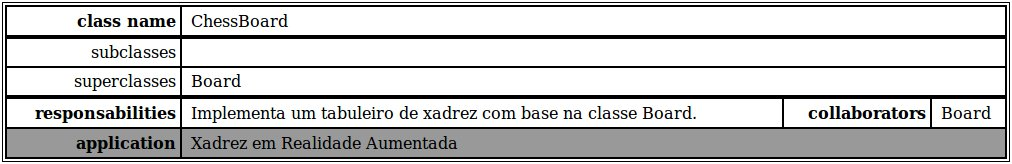
\includegraphics[width=1.0\textwidth]{crc/ChessBoard}
	    \end{figure}
      \subsubsection{ChessPiece}
      \label{subsubsec:crcchesspiece}
      \begin{figure}[H]
	    \centering
	    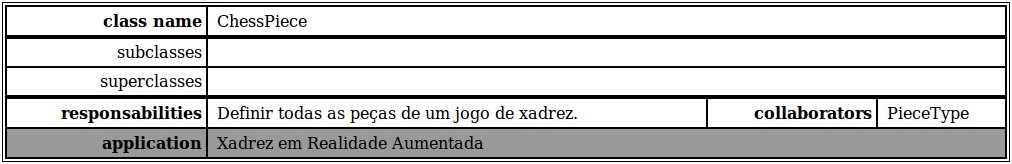
\includegraphics[width=1.0\textwidth]{crc/ChessPieces}
	    \end{figure}
      \subsubsection{Validator}
      \label{subsec:crcvalidator}
      \begin{figure}[H]
	    \centering
	    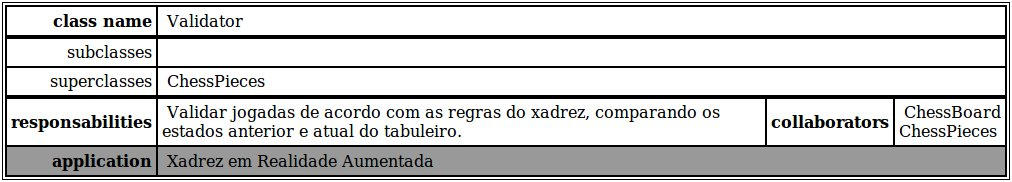
\includegraphics[width=1.0\textwidth]{crc/Validator}
	    \end{figure}
      \subsubsection{DummyAI}
      \label{subsec:crcdummyai}
      \begin{figure}[H]
	    \centering
	    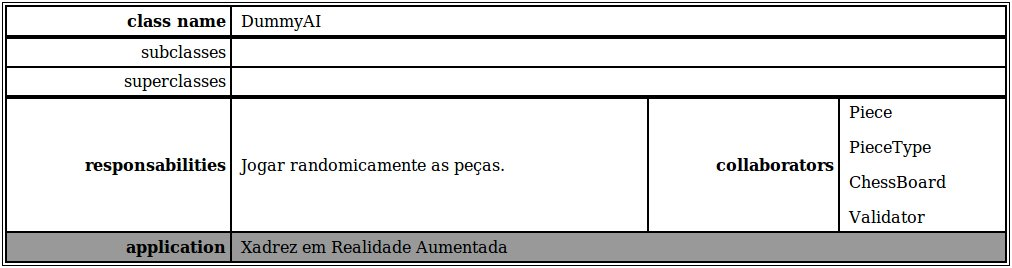
\includegraphics[width=1.0\textwidth]{crc/DummyAI}
	    \end{figure}
  \section{Pacote Interface}
  \label{sec:pacoteinterface}
    \subsection{ARCInterface}
    \label{subsec:crcarcinterface}
    \begin{figure}[H]
	  \centering
	  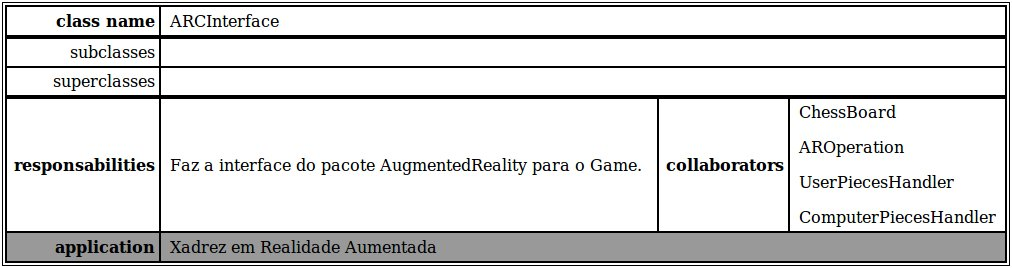
\includegraphics[width=1.0\textwidth]{crc/ARCInterface}
	  \end{figure}
    \subsection{ComputerPiecesHandler}
    \label{subsec:crccomputerpieceshandler}
    \begin{figure}[H]
	  \centering
	  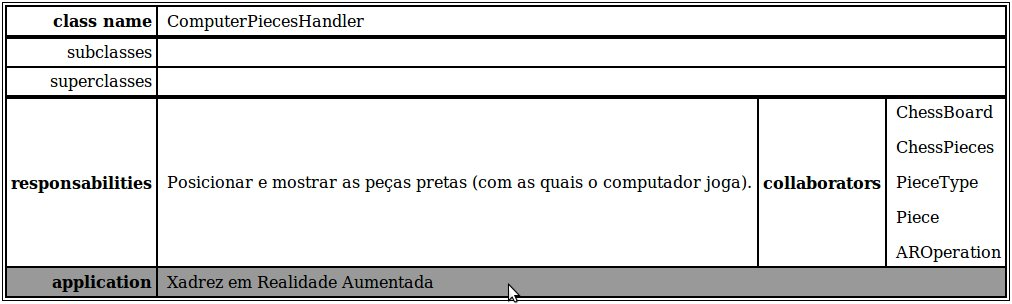
\includegraphics[width=1.0\textwidth]{crc/ComputerPiecesHandler}
	  \end{figure}
    \subsection{UserPiecesHandler}
    \label{subsec:crcuserpieceshandler}
    \begin{figure}[H]
	  \centering
	  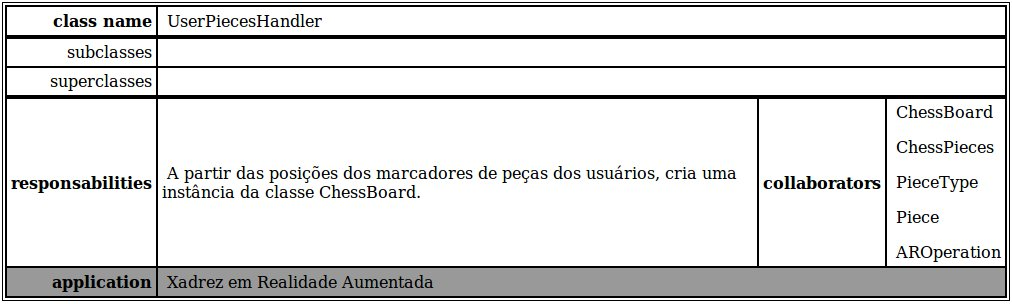
\includegraphics[width=1.0\textwidth]{crc/UserPiecesHandler}
	  \end{figure}
	\chapter{Prova de conceito}
	\label{ch:provadeconceito}
		\section{Introdu\c c\~ao}
		\label{sec:pcintroducao}
		A prova de conceito consistiu em abordar os pontos chave do projeto no que se
		refere a realidade aumentada. Nela, foram tratados temas como o reconhecimento
		de multiplos marcadores e a capacidade de obter as coordenadas do marcador no
		espa\c co. \footnote{A prova de conceito \'e o branch ``12 tags ao mesmo
		tempo" do reposit\'orio}
		
		\section{Marcadores}
		\label{sec:pcmarcadores}
		Na prova de conceito conseguimos com sucesso utilizar 12 marcadores quadrados
		com 3cm de lado\footnote{Uma casa de tabuleiro de xadrez oficial \'e um
		quadrado com, no m\'inimo, 5cm de lado e, no m\'aximo, 6,5cm de lado}. Demonstrando assim que
		o FLARManager consegue lidar com muitos marcadores, com tamanho pequeno e muito pr\'oximos, como ser\'a no
		nosso jogo.
		
		\section{Posi\c c\~ao do marcador no espa\c co}
		\label{sec:pcposicaodomarcadornoespaco}
		\'E fundamental conseguir identificar a posi\c c\~ao de um marcador no espa\c
		co, pois sem isso seria imposs\'ivel montar a matriz de pe\c cas no tabuleiro.
		Esta parte n\~ao apresentou problemas uma vez que sua \'unica dificuldade foi
		consultar a documenta\c c\~ao do FLARManager e descobrir que um objeto da
		classe FLARMarker possui os atributos p\'ublicos ``x'', ``y'' e ``z''. Com
		isso foi feito um m\'etodo na classe ARObject
		(\ref{subsec:crcarobject})para pegar estes atributos.
		
\end{document}
